% Packages
\documentclass[12pt]{article}
\usepackage[margin=2.5cm]{geometry}
\usepackage{lipsum}
\usepackage{titlesec, titletoc}
\usepackage[svgnames, table]{xcolor}
\usepackage{algorithm}
\usepackage{algpseudocode}
\usepackage{mdframed}
\usepackage[T1]{fontenc}
\usepackage{amsmath,amsthm,amsfonts,amssymb,mathtools}
\usepackage[osf]{mathpazo}
\usepackage{enumitem}

% Formating setup
\footskip = 1 cm
\setlength{\parindent}{0pt}
\pdfpxdimen=1in
\parindent = 0pt
\definecolor{myBlue}{RGB}{0, 81, 255}
\titleformat{\section}[block]{\sffamily\large\bfseries}{\thesection}{.5em}{\textcolor{myBlue}
{\titlerule[1.5pt]}\\\sffamily}[\vspace*{-3mm}\textcolor{myBlue}{\titlerule[1.5pt]}]
\titleformat{\subsection}{\large\sffamily\bfseries}{\thesubsection}{0.5em}{\textcolor{Black}}
\newcounter{boxedlistcounter}
\newenvironment{pseudo}{%
  \setcounter{boxedlistcounter}{0}% <-- Add this line to reset the counter
  \mdframed[
    linecolor=black, % color of the border
    linewidth=1.5pt, % thickness of the border
    roundcorner=10pt, % radius of the corners
    innertopmargin=0.6\baselineskip, % space at the top of the box
    innerbottommargin=0.6\baselineskip, % space at the bottom of the box
  ]
  \fontsize{12pt}{14pt}\selectfont % add font size command here
  \mdseries % add font series command here
}{%
  \endmdframed%
}
\newcommand{\I}{\par\stepcounter{boxedlistcounter}\arabic{boxedlistcounter}.\hspace{5pt}}
\newcounter{boxedlistcounter2}
\newenvironment{Proof}{%
  \refstepcounter{boxedlistcounter2}%
  \mdframed[
    linecolor=black, % color of the border
    linewidth=1.5pt, % thickness of the border
    roundcorner=10pt, % radius of the corners
    innertopmargin=\baselineskip, % space at the top of the box
    innerbottommargin=\baselineskip, % space at the bottom of the box
  ]
  \fontsize{12pt}{14pt}\selectfont % add font size command here
  \mdseries % add font series command here
}{%
  \endmdframed%
}
\newcommand{\PI}{\par\textbullet\hspace{5pt}}
\setlist[itemize]{itemsep=1pt}
\newcommand{\NL}{\par\hspace{12.5pt}}
\setlist[itemize]{itemsep=1pt}

% Custom commands
\newcommand{\for}[1]{\textbf{for} #1 \textbf{do}}
\newcommand{\IF}[1]{\textbf{if} #1 \textbf{then}}
\newcommand{\ELIF}[1]{\textbf{else if} #1 \textbf{then}}
\newcommand{\ELSE}{\textbf{else}}
\newcommand{\return}[1]{\textbf{return} #1}
\newcommand{\assign}{ $\leftarrow$ }
\newcommand{\DEF}[2]{\textbf{def} #1(#2):}
\newcommand{\1}{\space \quad}
\newcommand{\2}{\quad \quad \quad}
\newcommand{\3}{\quad \quad \quad \quad \space}
\newcommand{\4}{\quad \quad \quad \quad \quad \quad}
\newcommand{\comment}[1]{\hfill \textit{\# #1}}
\newcommand{\while}[1]{\textbf{while} #1 \textbf{do}}


% Document start ------------------------------------------------------------------------------------
\begin{document}

% Section 1  ----------------------------------------------------------------------------------------
\section{Priority Queue ADT}
Priority Queues are a special type of ADT that stores maps of key-value items where we can remove the smallest or the 
largest item in a min or max PQ respectively.
\begin{itemize}
  \item insert(k,v): Inerts itme with key k and value v.
  \item remove\_ming()/remove\_max(): Removes \& returns the item with smallest/largest key.
  \item min()/max(): Returns item with the smallest/largest key.
  \item size():Returns how many items are stored.
  \item is\_empty(): Tests of queue is empty.
\end{itemize}

\subsection{Sequence based Priority Queue}
\textbf{Unsorted list implementation}
\begin{itemize}
  \item insert runs in O(1) time since we can insert the item at the beginning or end of the sequence.
  \item remove\_min and min and their equivalents run in O(n) time since we have to traverse the entire list to find the smallest key.
\end{itemize}
\textbf{Sorted list implementation}
\begin{itemize}
  \item insert runs in O(n) time since we have to find the correct place in the order to insert the item.
  \item remove\_min and min and their equivalents run in O(1) time since the smallest key is at the beginning.
\end{itemize}

% Section 2  ----------------------------------------------------------------------------------------
\section{Priority Queue Sorting}
We can use a priority queue to sort a list of keys. To do so, first iteratively insert keys into an empty PQ. Then iteratively
remove\_min to get the keys in sorted order. Either sequeunce based implementation takes O($n^2$).
\newpage
\begin{pseudo}
  \I \DEF{priority\_queue\_sorting}{A}
  \I \1 pq \assign \textbf{new} priority queue
  \I \1 n \assign size(A)
  \I \1 \for{i in [$0$:n] do}
  \I \2 pq.insert(A[i])
  \I \3 pq.insert(A[i])
  \I \2 \for{i in [$0$:n]}
  \I \3 A[i] = pq.remove\_min()
\end{pseudo}

\subsection{Selection Sort}
Selection sort is a variant of pq sort that uses unsorted sequence implementation. The algorithm works by first inserting elements with n 
insert operations which takes O(n) time. It them removes elements with n remove\_min operations which takes O($n^2$).
\begin{pseudo}
  \I \DEF{selection\_sort}{A}
  \I \1 n \assign size(A)
  \I \1 \for{i in [$0$:n]} \comment{find s >= i minimizing A[s]}
  \I \2 s \assign i
  \I \2 \for{j in [i:n]}
  \I \3 \IF{A[j] < A[s]}
  \I \4 s \assign j
  \I \2 A[i], A[s] \assign A[s], A[i] \comment{swap A[i] and A[s]}
\end{pseudo}

\subsection{Insertion Sort}
Variant of pq-sort using sorted sequence implementation that first inserts eleemnts with n insert operations which takes O($n^2$) time
before removing elements with n remove\_min operations which takes O(n) time.
\begin{pseudo}
  \I \DEF{insertion\_sort}{A}
  \I \1 n \assign size(A)
  \I \1 \for{i in [1:n]}
  \I \2 x \assign A[i] \comment{move forward entries > x}
  \I \2 j \assign i
  \I \2 \while{j > $0$ and x < A[j-1]}
  \I \3 A[j] \assign A[j-1]
  \I \3 j \assign j -1 \comment{if x>0,  x >= A[j-1]}
  \I \2 A[j] \assign x \comment{if j<i,  x < A[j+1]}
\end{pseudo}

% Section 3  ----------------------------------------------------------------------------------------
\newpage
\section{Heap data structure (min-heap)}
A heap is a binary tree stroing (key. value) items at its nodes. It satisifies the properties:
\begin{itemize}
  \item Heap-order: for every node m \!= root, key(m) >= key(parent(m))
  \item Complete Binary Tree: let h be the height. Eevery level i < h is full (i.e., there are 2i nodes). Remaining nodes take leftmost positions of level h.
\end{itemize}
\vspace{10pt}
\textbf{RTP:} The root always holds the smallest key in the heap
\begin{Proof}
  \PI Suppose the minimum key is at some internal node x.
  \PI Because of the heap property, as we move up the tree, the keys can only get smaller 
  \NL (assuming repeats, otherwise contradiction)
  \PI If x is not the root, then its parent must hold a smaller key.
  \PI Keep going until we reach the root.
\end{Proof}
\vspace{10pt}
\textbf{RTP:} A heap storing n keys has height log n
\begin{Proof}
  \PI Let h be the height of a heap storing n keys
  \PI Since there are $2^i$ keys at depth i = 0, … , h - 1 and at least one key at depth h, we 
  \NL have n >= 1 + 2 + 4 + … + 2h-1 + 1
  \PI Thus, n >= 2h , applying log2 on both sides, log2 n >= h
\end{Proof}

\subsection{Insertion into a Heap}
Firstly, create a new node with the given key. Fine location for new node. Restore the heap-order property.

\vspace{10pt}
\subsection{Upheap} 
Restore heap-order property by swapping keys along the upward path.
\begin{pseudo}
  \I \DEF{up\_heap}{z} \comment{O(log(n))}
  \I \1 \while{z != root and key(parent(z)) > key(z)}
  \I \2 swap key of z and parent(z)
  \I \2 x \assign parent(z)
\end{pseudo}

\subsection{Finding the position for insertion: O(log n)}
\begin{itemize}
  \item Start from the last node
  \item Go up until a left child or the root is reached
  \item If we reach the root then need to open a new level
  \item Otherwise, go to the sibling (right child of parent)
  \item Go down left until a leaf is reached
\end{itemize}
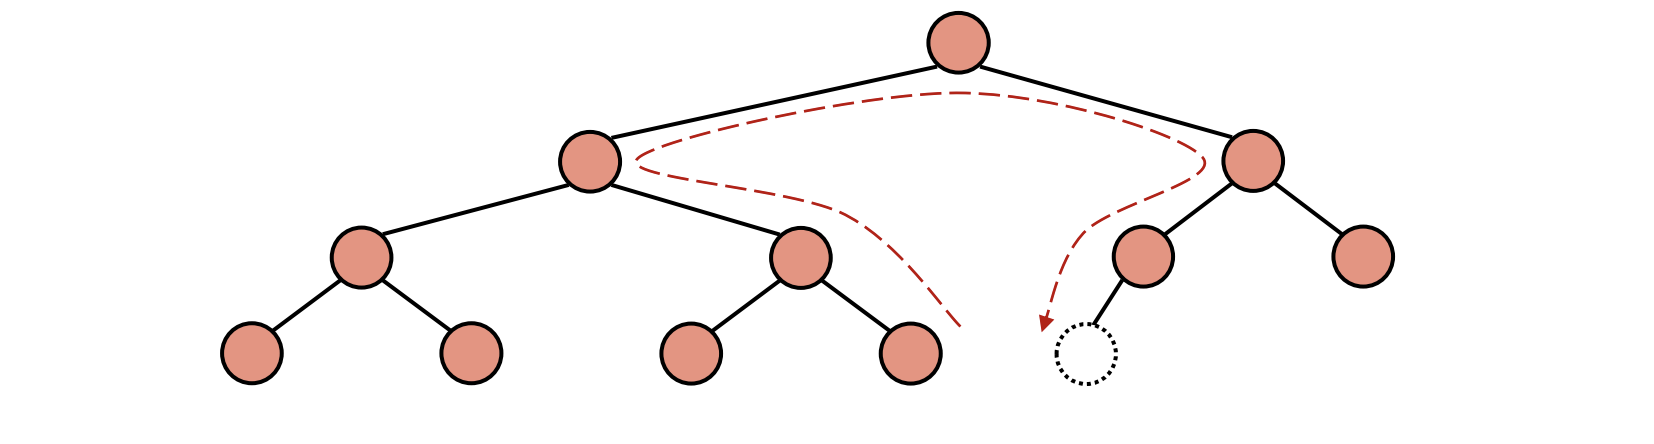
\includegraphics[width=\textwidth]{image10.png}

\subsection{Removal from a heap}
Replace the root key with the key of the last node w. Delete w. Restore the heap-order property

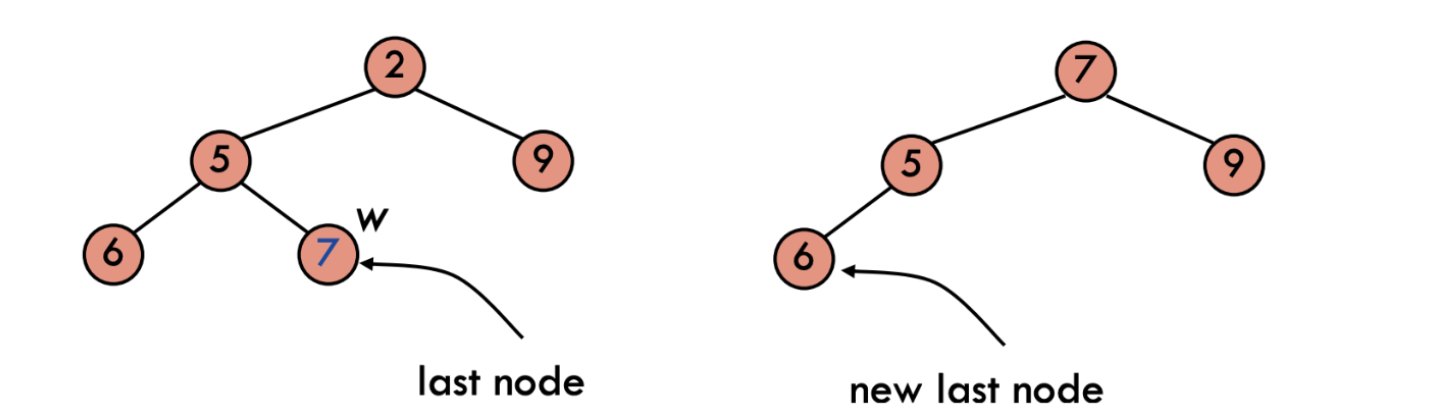
\includegraphics[width=\textwidth]{image11.png}

\subsection{Downheap}
Restore heap-order property by swapping keys along downward path from the root.

\begin{pseudo}
  \I \DEF{down\_heap}{z} \comment{O(log(n))}
  \I \1 \while{z has child with key(child) < key(z)}
  \I \2 x \assign child of z with the smallest key
  \I \2 x \assign parent(z)
  \I \2 z \assign x \comment{swap keys of z and x}
\end{pseudo}

% Section 4  ----------------------------------------------------------------------------------------
\newpage
\section{Heap-Sort}
Consider a priority queue with n items implemented with a heap: the space used is O(n) methods insert and remove\_min take O(log n).
Heap-sort is the version of priority-queue sorting that implements the priority queue with a heap. It runs in O(n log n) time.

\subsection{Heap-in-array implementation}
We can represent a heap with n keys by means of an array of length n.

\begin{itemize}
  \item The root is at $0$.
  \item The last node is at n-1.
  \item The left child of i is at index 2i+1.
  \item The right child of i is at index 2i+2.
  \item The parent of i is at index floor((i-1)/2).
\end{itemize}

\subsection{Summary of Heap-Sort}
Heap-sort can be arranged to work in place using part of the array for the output and part for the priority queue
\textcolor{blue}{A heap on n keys can be constructed in O(n)} time. But the n remove\_min still take O(n log n) time. Some other operations include:
\begin{itemize}
  \item remove(e): Remove item e from the priority queue.
  \item replace\_key(e, k): Update key of item e with k.
  \item replace\_value(e, v): Update value of item e with v.
\end{itemize}

\begin{tabular}{|l|l|l|l|}
  \hline
  \rowcolor{myBlue}
  \color{white}{\textbf{Method}} \hspace{60pt} & \color{white}{\textbf{Unsorted List}} \hspace{40pt} & \color{white}{\textbf{Sorted List}} \hspace{40pt} & \color{white}{\textbf{Heap}} \hspace{60pt} \\
  \hline
  size, isEmpty & O(1) & O(1) & O(1) \\
  \hline
  insert & O(1) & O(n) & O(logn) \\
  \hline
  min & O(n) & O(1) & O(1) \\
  \hline
  removeMin & O(n) & O(1) & O(logn) \\
  \hline
  remove & O(1) & O(1) & O(logn) \\
  \hline
  replaceKey & O(1) & O(n) & O(logn) \\
  \hline
  replaceValue & O(1) & O(1) & O(1) \\
  \hline
\end{tabular}










\end{document}